\documentclass{article}
\usepackage[utf8]{inputenc}
\usepackage[T1]{fontenc}
\usepackage{polski}
\usepackage{indentfirst}
\usepackage{lastpage}
\usepackage{fancyhdr}
\usepackage{graphicx}
\usepackage{listings}
\usepackage{caption}
\captionsetup[figure]{name={Rysunek}}

\pagestyle{fancy}
\fancyhf{}
\rhead{ Franciszek Wysocki, Bartosz Zdybel}
\rfoot{Strona \thepage \hspace{1pt} z \pageref{LastPage}}

\title{Specyfikacja implementacyjna gry w czołgi \\ pt. „BattleZone”}
\author{}
\date{}

\begin{document}
\maketitle

\begin{flushright}
\par ...
\vfill
\par
Wykonali: Franciszek Wysocki, Bartosz Zdybel

Sprawdzający: mgr inż. Paweł Zawadzki

Data: 19.04.2020
\end{flushright}

\thispagestyle{empty}
\newpage


\begin{frame}{}
    \tableofcontents
\end{frame}
\lhead{Spis treści}
\newpage

\section{Cel dokumentu}
\lhead{Cel dokumentu}

Dokument ten przedstawia szczegóły dotyczące implementacji gry w czołgi pt. „BattleZone” oraz wytyczne dotyczące wersjonowania, środowiska, testów, bibliotek itd... 

\section{Cel projektu i informacje ogólne}

Celem projektu jest stworzenie gry/programu, który będzie posiadał graficzny interfejs użytkownika (Grapical User Interface, GUI). Wymagane dane będą odczytywane z pliku konfiguracyjnego o rozszerzeniu txt. Program będzie sprawdzał poprawność wprowadzonych danych i na ich podstawie uruchomi grę, podczas której dwóch graczy bedzie rywalizować o zdobycie jak największej liczby punktów. (Więcej o zasadach gry opisane zostało w dokumencie ,,Specyfikacja funkcjonalna'').


\section{Środowisko deweloperskie}
Program będzie tworzony równolegle:
\begin{itemize}
\item na komputerze Dell Inspiron 5584 z procesorem Intel(R) Core(TM) i7-8565U CPU @ 1.80Ghz 1.99Ghz z pamięcią RAM 16 GB działającym na systemie Windows 10 Home (Wersja 10.0.18362.657) za pomocą środowiska IntellJ IDEA Community Edition 2019.3.2.
\item na komputerze Dell Vostro i7 z procesorem Intel(R) Core(TM) i7-8565U CPU @ 1.80Ghz 1.99Ghz z pamięcia RAM 8 GB działającym na systemie Windows 10 Pro za pomocą środowiska IntellJ IDEA Community Edition 2019.3.3.
\end{itemize}

Kod będzie pisany w języku java.

\section{Zasady wersjonowania}

Wersjonowanie odbędzie się za pomocą gita (w formie dodanych tagów):

\begin{itemize}
\item
,,STABLE\_n'' - wersje stabilne, gdzie n = 1.0, 2.0, ...,
\item
,,FINAL\_RELEASE'' - wesja finalna,
\end{itemize} 


Wiadomości z ,,commitów'' będą pisane w języku angielskim i będą opisywały co zostało dodane/zmienione od czasu poprzedniego commita (z danego brancha).

Np. Added an InputFileReader class.

Praca na modułach będzie odbywać sie równolegle na gałęziach. Do scalania wykorzystywane będzie polecenie git merge.


\section{Klasy}
\lhead{Opis klas}
\subsection{Opis klas}
W programie zostaną wyróżnione poniższe klasy:
\begin{itemize}
\item Game - główna klasa w grze (dziedzicząca po klasie JFrame). Zostanie w niej umieszczona metoda main. Klasa ta będzie odpowiadać za sterowanie grą. Znajdzie się w niej pętla, która co określony czas będzie wywoływać metody renderujące obraz i aktualizujące poszczególny stan gry.

\item MenuPanel - panel startowy (dziedziczący po klasie JPanel). Będzie to pierwszy panel, który pojawi się po uruchomieniu programu. Użytkownicy będą musieli wprowadzić w nim maksymalny czas przewidziany na grę, a także będą mogli wprowadzić w nim swoje imiona/nicki.

\item GamePanel - główny panel gry (dziedziczący po klasie JPanel). Będzie to docelowy panel, na którym będzie odbywać się rozgrywka. Dodatkowo będzie się na nim wyświetlał pozostały czas gry, zdobyte punkty itd... Klasa ta będzie posiadać między innymi metodę zapisującą ostatni stan planszy do pliku.

Powyższe panele będą połączone za pomocą klasy CardLayout.

\item Cell - klasa reprezentująca komórkę (dziedzicząca po klasie Rectangle). Będzie posiadała przede wszystkim pola z bieżacą wartością, bieżącym spritem (prostokąt w odpowiednim kolorze z odpowiednią wartością), informacje o jej punktach spadkowych oraz o tym czy jest komórką Armagedon. Klasa Rectangle zapewni pola położenia i rozmiar. Dodatkowo klasa będzie posiadać między innymi metody do zwięszania/zmniejszania wartości, zmniejszania rozmiaru itd...

\item Cells - klasa obsługująca i przechowująca komórki. Bedzie ona miała metody pozwalające na generowanie nowych komórek (zwykłych i komórek-dzieci), zmniejszania rozmiaru/zwiększania wartości całej populacji itd... Będzie ona posiadać także metodę sprawdzającą czy któryś z pocisków trafił w którąś komórkę i wykonywać odpowiednie dla tego działania.

\item Bullet - klasa reprezentująca pocisk (dziedzicząca po klasie Rectangle). Będzie ona posiadać informacje o współrzędnych miejsca wystrzelenia, kierunku, prędkości itd...
Będzie posiadać między innymi metodę, która zaktualizuje położenie pocisku.

\item Player - klasa abstrakcyjna reprezentująca gracza. Bedzie posiadać tablicę sprite'ów z czołgami (z różnie ustawioną lufą), współrzędne położenia, będzie takżę przechowywać listę nabojów, którą wystrzelił dany gracz. Będzie posiadała kilka metod abstrakcyjnych (np. sterujące) oraz kilka napisanych domyślnie takich jak np. kasowanie pocisku z listy, gdy ten wyleci za plasze.

\item LeftPlayer/RightPlayer - klasy reprezentujące odpowiednio lewego i prawego gracza (dziedziczące po klasie Player). Będą posiadały przede wszystkim metody sterujące czołgami. 

\item KeysListener - klasa odpowiadajace za obsługę klawiszy (implementująca interfejs KeyListener). Będzie posiadała metody sprawdzające czy dany klawisz został naciśnięty.

\item InputFileReader - klasa odpowiadająca za odczytywanie danych z pliku konfiguracyjnego. Będzie przechowywać wszystkie stałe wartości w grze.

\end{itemize}
\lhead{Diagram klas}
\subsection{Diagram klas}
\begin{figure} [hbt!]
    \centering
    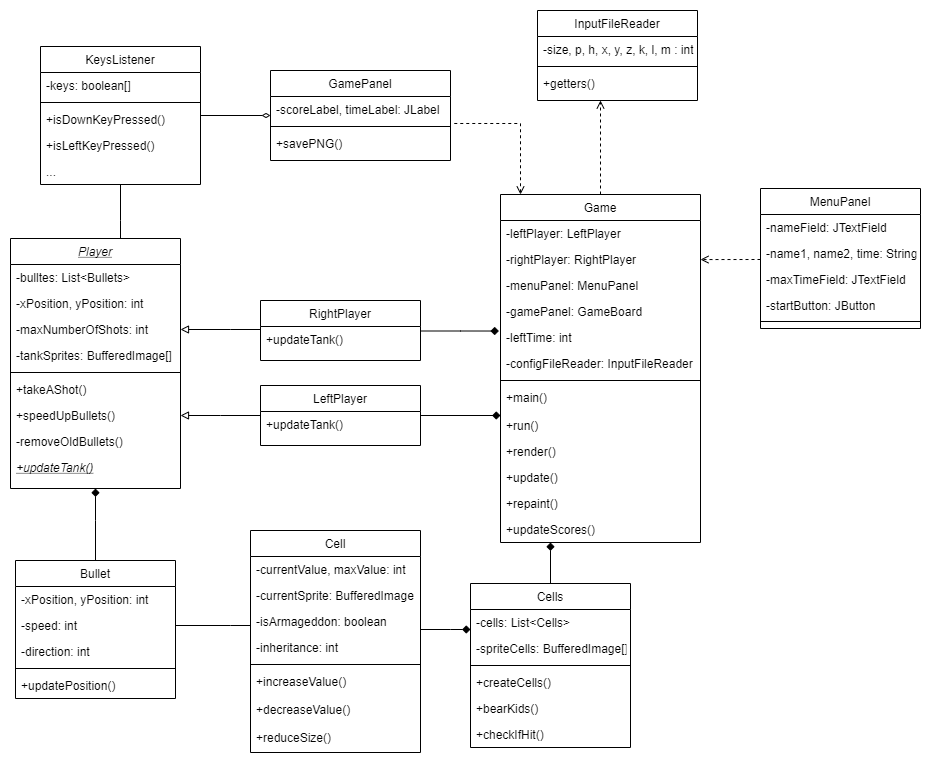
\includegraphics[width=13cm]{DiagramKlas.png}
   \captionof{figure}{}
\end{figure}


\newpage

\section{Argumenty wywołania}


Podczas uruchamiania będzie można podać nazwę pliku wejściowego z rozszerzeniem txt.

Podanie innego argumentu niż nazwa pliku spowoduje przerwanie działania programu i wyświetlenie stosownego komunikatu.

W przypadku uruchomienia programu bez podania nazwy zostanie wczytany domyślny plik konfiguracyjny.
\lhead{Argumenty wywołania}
\section{Testowanie}

Program będzie zawierał testy jednostkowe. Będą one pisane na bieżąco powstawania kodu i będą dotyczyły sprawdzania konkretnych funkcjonalności. Do ich pisania zostanie wykorzystana biblioteka AssertJ, a do ich automatycznego uruchamiania narzędzie jakim jest Maven. Wszystkie testy będą znajdować się w katalogu tests a ich nazwy będą tworzone zgodnie z poniższą konwencja nazewnicza:

TestNazwaKlasyTestowanej

np. TestCell


\section{Biblioteki}
\begin{itemize}
    \item Testowanie (jak wspomniano wyżej) będzie oparte na bibliotece AssertJ. 

    \item Graficzny interfejs użytkownika będzie oparty na bibliotece graficznej Swing.
\end{itemize}


\section{Struktury danych}

Zarówno wystrzelone pociski, jak i aktywne komórki będą przechowywane za pomocą struktury danych zwanej listą. Wykorzystany zostanie interfejs List (\texttt{java.util.List}), a konkretnie jego podtyp LinkedList, dzięki temu zarówno dodowanie (np. wystrzelenie pocisku), jak i odejmowanie obiektów (np. komórki po zestrzeleniu) będzie szybsze niż np. dla tablicy lub klasy ArrayList, które musiałaby przesuwać inne obiekty w pamięci, aby się dostosować. Poza tym nie będzie potrzeby korzystania z dostępu do konkretnych elementów (w przypadku komórek ich kolejność będzie w dodatku losowa) z jakiej słyną wspomniana tablica i klasa ArrayList, dlatego, że co określony czas będzie nastąpowała iteracja po całej kolekcji np. żeby sprawdzić czy którykolwiek pocisk nie wleciał w którąkolwiek komórkę.

Sprite'y (ang. Sprites) będą przechowywane za pomocą tablic. Nie będzie modyfikowana ich kolejność, nie będą dodawane nowe, ani kasowane stare, będzie natomiast ważny szybki dostęp.


\section{Algorytmy}

\begin{enumerate}
    \item Algorytm sprawdzania czy którykolwiek pocisk wleciał w którąkolwiek komórkę.

W tym celu co określony czas nastąpi iteracja po liście komórek i dla każdej komórki nastąpi iteracja po liście pocisków.
Zarówno pociski, jak i komórki będą dziedziczyły po klasie Rectangle, dzięki czemu będzie możliwe wykorzystanie poniższych metod tej klasy (Rysunek 2) do sprawdzenia czy pocisk trafił w komórkę:

\begin{figure} [hbt!]
    \centering
    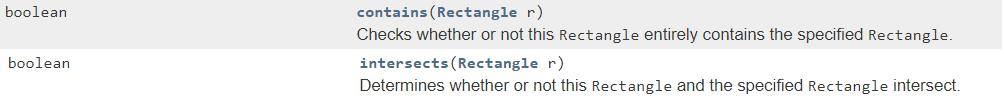
\includegraphics[width=13cm]{javaDoc.png}
   \captionof{figure}{Źródło: https://docs.oracle.com/javase/7/docs/api/index.html}
\end{figure}


 \item Algorytm określania miejsca wystrzału i kierunku lotu pocisku.
 
 W momencie wystrzału będzie pobierana wysokość czołgu w danej chwili oraz indeks jego obecnego sprite'a (te w tablicy będą posortowane według wysokości lufy). Miejsce wystrzału będzie określane zatem biorąc wysokość czołgu i dodając/odejmując wielokrotność indexu. Przyrost wysokości pocisku (kierunek) będzie natomiast określany na podstawie odchylenia indexu sprite'u od środkowego.
 
 
  \item Algorytm zmniejszania rozmiaru komórek.
  
Oprócz zmienienia samych wymiarów (szerokości i wysokości) oraz skalowania Sprite'a danej komórki, będzie ona dodatkowo ustawiana w centrum powierzni, którą zajmowała przed zmniejszeniem.
Zatem do współrzędnej położenia x będzie dodawana połowa różnicy między starą, a obecną szerokością. Analogicznie dla współrzednej y, będzie dodawana połowa różnicy między starą, a obecną wysokością.
 
 \lhead{Algorytmy}
\end{enumerate}
\end{document}

